\documentclass{anstrans}
%%%%%%%%%%%%%%%%%%%%%%%%%%%%%%%%%%%
\title{Extension of the entropy viscosity method to the low-Mach regime for the multi-dimensional Euler equations}
\author{Marc O. Delchini$^{*}$, Jean C. Ragusa$^{*}$, Ray A. Berry$^\dagger$}

\institute{
$^{*}$Department of Nuclear Engineering, Texas A\&M University, 
$^\dagger$Idaho National Laboratory
}

\email{delchmo@tamu.edu \and jean.ragusa@.tamu.edu \and ray.berry@inl.gov}

% Optional disclaimer: remove this command to hide
%\disclaimer{Notice: This manuscript is a work of fiction. Any resemblance to actual articles, living or dead, is purely coincidental.}

%%%% packages and definitions (optional)
\usepackage{graphicx} % allows inclusion of graphics
\usepackage{booktabs} % nice rules (thick lines) for tables
\usepackage{microtype} % improves typography for PDF
%\usepackage{subfigure}
\usepackage{subcaption}
\usepackage{float}


\renewcommand{\div}{\vec{\nabla}\! \cdot \!}
\newcommand{\grad}{\vec{\nabla}}
\newcommand{\divv}[1]{\vec{\nabla}^{#1}\! \cdot \!}
\newcommand{\gradd}[1]{\vec{\nabla}^{#1}}
% latex shortcuts
\newcommand{\bea}{\begin{eqnarray}}
\newcommand{\eea}{\end{eqnarray}}
\newcommand{\be}{\begin{equation}}
\newcommand{\ee}{\end{equation}}
\newcommand{\bal}{\begin{align}}
\newcommand{\eali}{\end{align}}
\newcommand{\bi}{\begin{itemize}}
\newcommand{\ei}{\end{itemize}}
\newcommand{\ben}{\begin{enumerate}}
\newcommand{\een}{\end{enumerate}}
% DGFEM commands
\newcommand{\jmp}[1]{[\![#1]\!]}                     % jump
\newcommand{\mvl}[1]{\{\!\!\{#1\}\!\!\}}             % mean value
\newcommand{\keff}{\ensuremath{k_{\textit{eff}}}\xspace}
% shortcut for domain notation
\newcommand{\D}{\mathcal{D}}
% vector shortcuts
\newcommand{\vo}{\vec{\Omega}}
\newcommand{\vr}{\vec{r}}
\newcommand{\vn}{\vec{n}}
\newcommand{\vnk}{\vec{\mathbf{n}}}
\newcommand{\vj}{\vec{J}}
\newcommand{\eig}[1]{\| #1 \|_2}

\newcommand{\EI}{\mathcal{E}_h^i}
\newcommand{\ED}{\mathcal{E}_h^{\partial \D^d}}
\newcommand{\EN}{\mathcal{E}_h^{\partial \D^n}}
\newcommand{\ER}{\mathcal{E}_h^{\partial \D^r}}
\newcommand{\reg}{\textit{reg}}

\newcommand{\norm}{\textrm{norm}}
\renewcommand{\Re}{\textrm{Re}}
\newcommand{\Pe}{\textrm{P\'e}}
\renewcommand{\Pr}{\textrm{Pr}}

\newcommand{\resi}{R_e}
%\newcommand{\resinew}{\tilde{D}_e}
\newcommand{\resinew}{\widetilde{\resi}}
\newcommand{\matder}[1]{\frac{\textrm{D} #1}{\textrm{D} t}}


% extra space
\newcommand{\qq}{\quad\quad}
% common reference commands
\newcommand{\eqt}[1]{Eq.~(\ref{#1})}                     % equation
\newcommand{\fig}[1]{Fig.~\ref{#1}}                      % figure
\newcommand{\tbl}[1]{Table~\ref{#1}}                     % table
\newcommand{\sct}[1]{Section~\ref{#1}}                   % section
\newcommand{\app}[1]{Appendix~\ref{#1}}                   % appendix

\newcommand\br{\mathbf{r}}
%\newcommand{\tf}{\varphi}
\newcommand{\tf}{b}


\begin{document}
%%%%%%%%%%%%%%%%%%%%%%%%%%%%%%%%%%%%%%%%%%%%%%%%%%%%%%%%%%%%%%%%%%%%%%%%%%%%%%%%
\section{Introduction}

We extend the entropy viscosity method, proposed by Guermond et al. \cite{jlg1, jlg2}
to low-Mach flows. The entropy viscosity technique is a viscous regularization technique
that satisfies the entropy minimum principle; adequate dissipation terms (viscous fluxes)
are added to the governing laws while ensuring the entropy minimum principle still holds.
Viscosity coefficients modulates the magnitude of the added dissipation such that it is
large in shock regions and vanishingly small elsewhere. The entropy viscosity coefficients
are taken proportional to the entropy production while, at the same time, being bounded
from above by a first-order viscosity coefficient that reduces the spatial discretization
to be similar to a first-order Godunov scheme (the latter being known to be overly dissipative but
monotone \cite{toro}). Hence, entropy production in shocks will result in large viscosity  
coefficients and thus will avoid spurious oscillations. 

The entropy method is independent of the type of spatial discretization (finite volume,
continuous or discontinuous finite elements, ...) and thus can be applied ubiquitously. 
For instance, it is currently being considered as one possible stabilization approach in 
RELAP-7, the next-generation reactor system code build upon the MOOSE multiphysics framework
\cite{moose}. However, it has mostly been tested for supersonic applications but not in low-Mach 
or transonic applications.  

In this summary, we show that current entropy production residual definition is undetermined 
in low-Mach regime and review an alternate and more suitable expression. Numerical results in 
low-Mach flows are presented.

%%%%%%%%%%%%%%%%%%%%%%%%%%%%%%%%%%%%%%%%%%%%%%%%%%%%%%%%%%%%%%%%%%%%%%%%%%%%%%%%
\section{Theory}

We recall the Euler equations with viscous regularization based on the entropy viscosity 
method:
\begin{subequations}
\label{eq:euler_visc}
%
\begin{equation}
\partial_t \rho  + \div \left( \rho \vec{u} \right) = \div \left( \kappa \grad \rho \right) 
\end{equation}
%
\begin{equation}
\partial_t \left( \rho \vec{u} \right) + \div \left( \rho \vec{u} \otimes \vec{u} + P \mathbf{I} \right) = \div \left( \mu \rho \grad^s \vec{u}  + \kappa \vec{u} \otimes \grad \rho \right)  
\end{equation}
%
\begin{equation}
\partial_t \left( \rho E \right) + \div \left[ \vec{u} \left( \rho E + P \right) \right] = \div \left( \kappa \grad \left( \rho e \right) + \frac{1}{2}|| \vec{u} ||^2 \kappa \grad \rho +  \rho \mu \vec{u} \grad \vec{u}  \right) 
\end{equation}
\end{subequations}
The notation is standard: $\rho$, $\rho \vec{u}$ and $\rho E$ are the density, the momentum and the total energy, respectively, and will be referred to as the conservative variables. $\vec{u}$ is the fluid velocity and its specific internal energy is denoted by $e=E-\tfrac{u^2}{2}$. The ideal gas equation of state is used to compute the pressure $P$.  $\kappa$ and $\mu$ are positive viscosity coefficients and are based on the local entropy production. These coefficients are numerically evaluated using the local entropy residual $\resi(\vec{r},t)$:
%
\begin{equation}
\label{eq:ent_residual}
\resi(\vec{r}, t) := \partial_t s + \vec{u} \cdot \grad s
\end{equation}
%
Then, the entropy viscosity coefficients are given by
\begin{subequations}
\label{eq:ent_visc_coeff}
\begin{equation}
\mu^K_e(\vec{r}_q,t) =  h_K^2 \frac{| \resi^K(\vec{r}_q,t) |}{|| s - \bar{s} ||_\infty}  
\end{equation}
\begin{equation}
\kappa^K_e(\vec{r}_q,t) = Pr \, \mu^K_e(\vec{r}_q,t)
\end{equation}
\end{subequations}
where $|| \cdot ||_\infty$ and $\bar{\cdot}$ denote the L$_\infty$-norm and the average operator over the entire computational domain, $K$ is a given element of the mesh, and $\vec{R}_q$ is a quadrature point location within cell $K$. $\Pr$ is the Prandtl number; see \cite{jlg1} for additional details..

However, in low-Mach regime, the flow is isentropic, so both the numerator and denominator in \eqt{eq:ent_visc_coeff} tend towards 0, making
the definition of the entropy viscosity coefficients ill-determined. One can recast demonstrate \cite{jlg,marco_inl_report} that
\begin{equation}
\label{eq:ent_res}
\resi(\vec{r},t) := \partial_t s + \vec{u} \cdot \grad s \propto \left( \matder{P} - c^2 \matder{\rho} \right)  :=\resinew(\vec{r},t) ,
\end{equation} 
where $\matder{\ }$ denotes the material derivative. Thus, one may use $\resinew$ instead of $\resi$ to evaluate the entropy production. Since the dynamics viscosity coefficients must have units of $m^2/s$, one can propose new normalization for $\resinew$ that can be appropriate in both low-Mach and supersonic regimes. For instance, we employ the following normalization
\be
M \rho \|\vec{u}\|^2 + (1-M) \rho c^2,
\ee
where $c$ is the speed of sound and the weighting factor is the local Mach number, $M=\|u\|/c$. Hence, the new entropy viscosity coefficients are given by:
\begin{subequations}
\label{eq:ent_visc_coeff2}
\begin{equation}
\mu^K_e(\vec{r}_q,t) =  h_K^2 \frac{| \resinew^K(\vec{r}_q,t) |}{M \rho \|\vec{u}\|^2 + (1-M) \rho c^2}  
\end{equation}
\begin{equation}
\kappa^K_e(\vec{r}_q,t) = Pr \, \mu^K_e(\vec{r}_q,t)
\end{equation}
\end{subequations}

%%%%%%%%%%%%%%%%%%%%%%%%%%%%%%%%%%%%%%%%%%%%%%%%%%%%%%%%%%%%%%%%%%%%%%%%%%%%%%%%
\section{Results and Analysis}

The Euler equation with viscous stabilization are discretized with {\it continuous} finite elements in space and BDF2 in time using MOOSE. The resulting nonlinear system of equations at each time step is solved using a Jacobian-free Newton Krylov technique. We present results a 2D flow over a circular hump \cite{Hump}. such problems are often employ to test the ability of a numerical scheme used in compressible  flow solvers to resolve low-Mach flows (i.e., in the incompressible limit)
\cite{LowMach1}. 

The results are shown in \fig{fig:2d_hump_mach_0p7}, \fig{fig:2d_hump_mach_0p01}, \fig{fig:2d_hump_mach_0p0001} and \fig{fig:2d_hump_mach_0p0000001} for inlet Mach numbers $M_{\infty}=0.7$, $M_{\infty}=0.01$, $M_{\infty}=10^{-4}$ and $M_{\infty}=10^{-7}$, respectively. It is expected that, within the low-Mach number range, the solution does not depend on the Mach number and is self-similar. The results showed in \fig{fig:2d_hump_mach_0p01}, \fig{fig:2d_hump_mach_0p0001} and \fig{fig:2d_hump_mach_0p0000001} correspond to the low-Mach regime. The iso-Mach lines are drawn ranging from the minimum and the maximum values (provided in each legend) using 50 equally-spaced intervals. The steady-state solution is symmetric and does not depend on the value of the inlet Mach number, as expected in the incompressible limit. 
%
For a flow at $M=0.7$, the compressible effects become more important and shock can form. An uniform grid of $3352$ $Q_1$ elements was used to obtain the numerical solution for Mach numbers below $M_{\infty}=0.01$. A once-refined mesh was employed for the $M_{\infty}=0.7$ simulation in order to better resolve the shock. A $CFL$ of 20 was employed and the simulations were run until steady state. 
%
In \fig{fig:2d_hump_mach_0p7}, the steady-state numerical solution develops a shock: the compressibility effect are no longer negligible. The iso-Mach lines are also plotted with $50$ intervals and range from $0.4$ to $1.6$. The shock is well resolved and does not display any instabilities or spurious oscillations. 
%
\begin{figure}[H]
        \centering
        \begin{subfigure}[b]{0.5\textwidth}
                \centering
                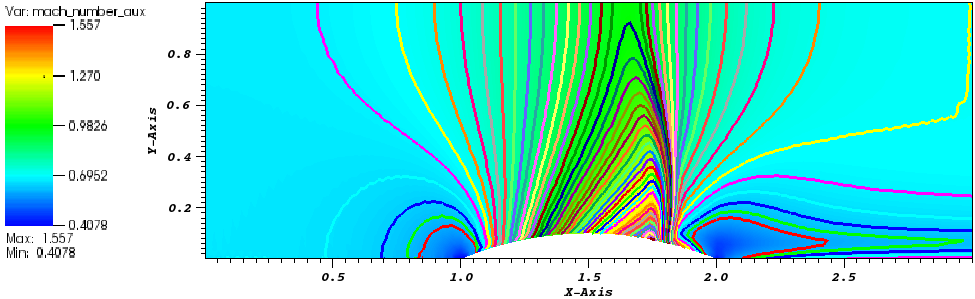
\includegraphics[width=\textwidth]{Hump2D_mach_0p7.png}
                \caption{Mach $0.7$}
                \label{fig:2d_hump_mach_0p7}
        \end{subfigure}%

        \begin{subfigure}[b]{0.5\textwidth}
                \centering
                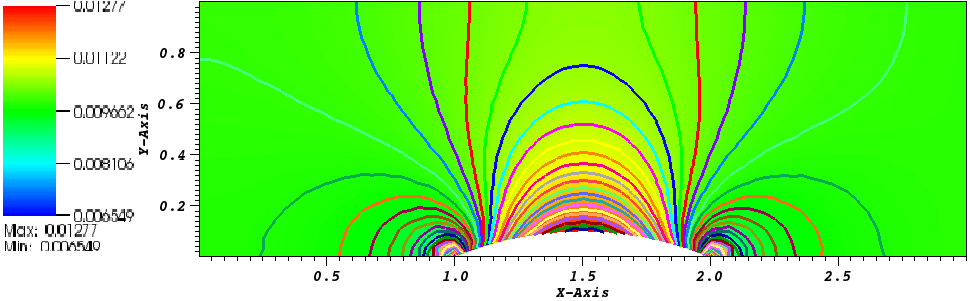
\includegraphics[width=\textwidth]{Hump2D_mach_0p01.png}
                \caption{Mach $10^{-2}$}
                \label{fig:2d_hump_mach_0p01}
        \end{subfigure}%
        
        \begin{subfigure}[b]{0.495\textwidth}
                \centering
                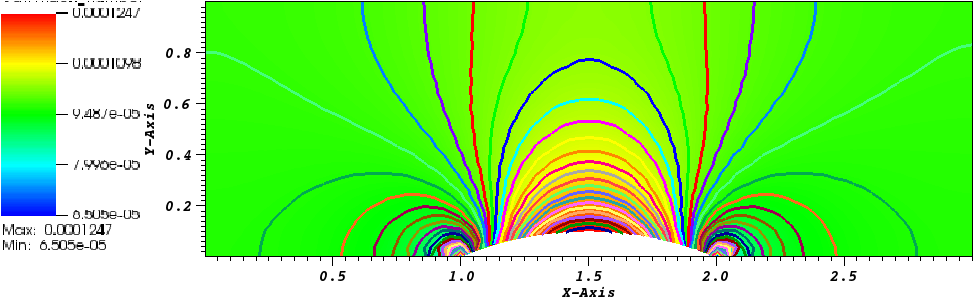
\includegraphics[width=\textwidth]{Hump2D_mach_1em4.png}
                \caption{Mach $10^{-5}$}
                \label{fig:2d_hump_mach_0p0001}
        \end{subfigure}

        \begin{subfigure}[b]{0.495\textwidth}
                \centering
                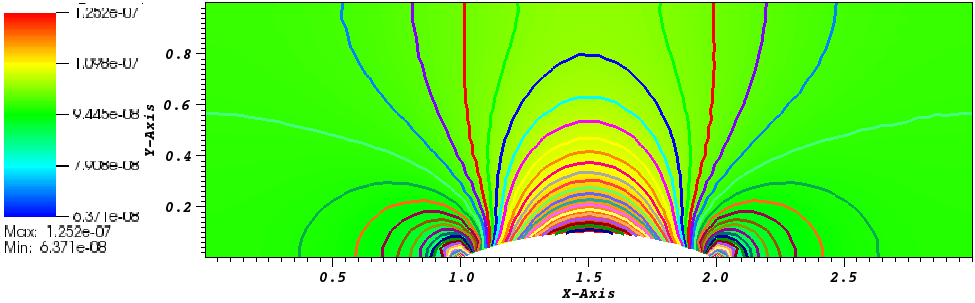
\includegraphics[width=\textwidth]{Hump2D_mach_1em7.png}
                \caption{Mach $10^{-7}$}
                \label{fig:2d_hump_mach_0p0000001}
        \end{subfigure}
        \caption{Iso-Mach lines for a 2-D flow over a circular bump (steady-state solution).}
				\label{fig:2d_hump}
\end{figure}
%
The results presented in \fig{fig:2d_hump} were obtained with the new definitions of the viscosity coefficients and illustrate the ability of the entropy viscosity method to correctly simulate several types of flows (subsonic and transonic flows) without tuning parameters. 


%%%%%%%%%%%%%%%%%%%%%%%%%%%%%%%%%%%%%%%%%%%%%%%%%%%%%%%%%%%%%%%%%%%%%%%%%%%%%%%%
\section{Conclusions}

We have presented an extension of the entropy viscosity method for low-Mach flows. In the future, we plan on adding heat generation, gravity, and friction terms. Another possible extension of this work (reported in these proceedings) deals with applying the entropy viscosity method to a 7-equation two-phase flow model. These steps will further contribute to the assessment of the stabilization technique for reactor flows.


%%%%%%%%%%%%%%%%%%%%%%%%%%%%%%%%%%%%%%%%%%%%%%%%%%%%%%%%%%%%%%%%%%%%%%%%%%%%%%%%
%\appendix
%\section{Appendix}

%%%%%%%%%%%%%%%%%%%%%%%%%%%%%%%%%%%%%%%%%%%%%%%%%%%%%%%%%%%%%%%%%%%%%%%%%%%%%%%%
%\section{Acknowledgments}
%This material is based upon work supported by the Department of Energy Rickover Fellowship Program in Nuclear Engineering.

%%%%%%%%%%%%%%%%%%%%%%%%%%%%%%%%%%%%%%%%%%%%%%%%%%%%%%%%%%%%%%%%%%%%%%%%%%%%%%%%
\bibliographystyle{ans}
\bibliography{bibliography}

\end{document}

